\documentclass[12pt]{article}
\usepackage[]{algorithm2e}
\usepackage{setspace}
\usepackage[margin=1in]{geometry}
\usepackage{graphicx}
\graphicspath{ {gfx/} }
\usepackage[capitalize]{cleveref}
\usepackage{subfig}
\usepackage{verbatim}

%\DeclareGraphicsExtensions{.pdf,.jpg,.png}
\doublespacing
\title{[Come up with title]}
\date{}
\begin{document}
	\maketitle


\section{Introduction}

\begin{figure}
\begin{center}
  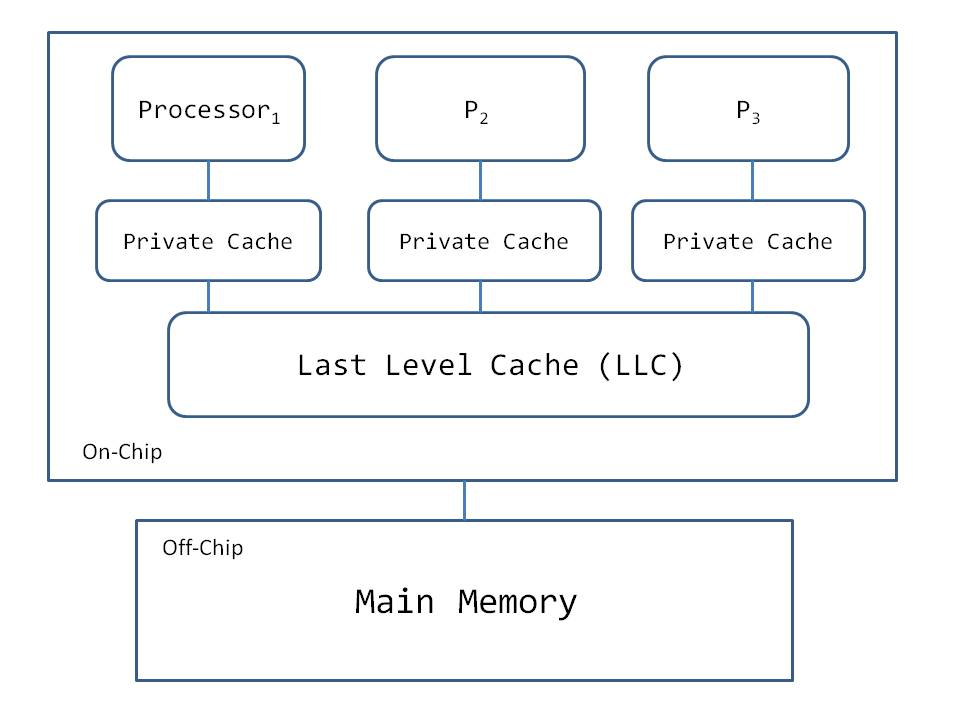
\includegraphics[width=10cm]{distributed_system.JPG}
  \caption{Simple diagram of a shared memory system.}
  \label{fig:distributed}
\end{center}
\end{figure}

In the modern day, there is a continuously increasing demand for faster computer processors. Since one of the most effective methods to address this is to add multiple cores to a CPU and allowing tasks to execute in parallel, the number of cores is increasing exponentially (a certain IBM chip contains 4,000 processor cores [cite?]). Multiple cores allow for tasks to be split up and handled simultaneously, but accurate and efficient performance requires parallelism and exploitation of shared memory. The essence of maintaining the “correctness” of data between cachelines is to prevent the use of stale data, which is old information that is being used when it has already been altered by another core. This problem is known as memory coherence, and a coherence protocol is necessary to facilitate performance and scalability of the system.

Memory coherence is most commonly and traditionally addressed by directory based coherence protocols [cite something], which is relatively intuitive. In such a system a central directory tracks the coherence between the caches, or how they are being owned or shared between cores. Thus, if a core requests private ownership of a cacheline, it must go through the directory so that all other lines can be invalidated and updated accordingly. Since the directory must maintain the sharer information for every cacheline, the system requires O(N) storage per cacheline if there are N cores. As N increases, the directory based protocol does not scale well.

This problem is addressed by Tardis, a new coherence protocol that is currently in development and has been mathematically proven to be sequentially correct [citation?]. Tardis utilizes logical timestamps (to be explained in more detail in Background) to enforce the global memory order. The protocol only requires O(log N) storage per cacheline and is therefore significantly more scalable as well as being simpler. However, the major disadvantages of the vanilla Tardis protocol is managing very large timestamps and dealing with potentially many renewal requests, most of which are unnecessary. 

The goal of this paper is to explore the expansive design space of Tardis and optimize the protocol through timestamp compression and renewal minimization. We implemented a clever base timestamp + delta scheme to reduce the storage overhead of timestamps, implemented and analyzed several configurations of lease protocols to reduce the number of renewals, and designed a livelock detection algorithm to prevent several worst-case-scenarios of spinning variables

\section{Background}
Tardis uses timestamps to logically organize shared memory and ensure coherence. It excels at being simple and very scalable. By operating with logical time instead of physical time, Tardis is able to have actions that seemingly “travel in time.” (Henceforth, time will refer to logical time.)

To give an analogy, think of a book in the library that two people want to read and then a third wants edit. Intuitively, it would seem that the two readers must first finish reading the book before the third person can edit, but Tardis allows all three people to perform their tasks at the same time (Need to verify this).  Using arbitrary but realistic numbers, the first person may read the book from logical time 0 to 10, the second person reads from 0 to 20, and the editor “travels in time” and starts editing the book at time 21.

This phenomenon is allowed to happen because of the use of timestamps to indicate logical time. Each cacheline, a basic unit of data storage, has two timestamps: Write Timestamp (WTS) and Read Timestamp (RTS). There is also a timestamp in each core called the Program Timestamp (PTS), which is only incremented when accessing data and should not be confused with the processor clock. PTS marks the core’s position in time and can vary between cores. RTS is always greater or equal to WTS, and the span of time between them dictates when the data is valid. This period is known as the lease because the core is basically reserving the information for a duration of time so that it will remain valid by specifying any change to that piece of data to be timestamped after the lease period. When a core’s PTS is in that range, the core may use that data, and when PTS is not, then the core must send a request to shared memory, known as the LLC, to request the newest version of the data, known as a renew request. If the WTS in the LLC is still the same, then the data has not been changed and the core can request another lease to keep using said data. If the data has been changed, then the renew request fails and the LLC sends back the newest version of the data.

The cachelines in shared memory can be in two states, shared and exclusive. A cachenline being in the shared state means that multiple cores can read from it. When a core wants to modify it, the cacheline is set to the exclusive state, signaling that it is exclusively owned by said core. When another core needs to read that cacheline, a writeback request is sent to the owner core, which then writes the updated data back to the LLCwith updated timestamps.

Take the following example:

[Picture of example here] http://people.csail.mit.edu/devadas/pubs/tardis.pdf

\begin{enumerate}
\setcounter{enumi}{-1}
	
\item The initial state of the two cores and two cachelines in the LLC
\item Cacheline A is moved into core 0 and the LLC registers that it is exclusively owned by core 0 since its value is being edited. PTS in core 0 is increased to 1 because an action, in this case changing its value to 1, is performed and thus it is advancing in logical time. 
\item pts of core 0 remains 1 because although cacheline B was loaded, no action was performed on it. B is only being read, so its rts increases to pts+10=11, where 10 is an arbitrarily picked lease value, to indicate a period of validity that lasts until pts exceeds 11. Methods of choosing lease will be discussed in the optimizations section. In the LLC, B’s timestamps and changed to reflect that it is being leased.
\item Core 1 needs to edit B, but that cacheline is currently being read by core 0, so when it puts B in the exclusive state, PTS, RTS, and WTS are all set to 11+1=12 to depict that core 1 is logically ahead of core 0. B’s timestamps show that the Bs in each core are existing at different places in logical time which means it having value of 0 in core 0 and a value of 1 in core 1 is perfectly valid. This is the phenomenon of “traveling in time” that is unique to Tardis because cacheline B is existing in different logical times at the same instant in physical time. 
\item Core 1 now needs to read A, so it leases the cacheline for 10 timestamps, which makes its RTS = 12+10 = 22 where 12 is the PTS of core 1 and 10 is the arbitrarily chose lease. Since it is now being read and not edited, its exclusive ownership by core 0 changes to shared ownership, as reflected in the timestamps in the LLC.
\end{enumerate}

\section{Optimizations} \label{sec:optimization}

In this section, we will detail the three optimizations we  have implemented to improve the efficiency and storage overhead of Tardis.

\subsection{Timestamp Compression}

One of the major structural changes implemented in Tardis is the inclusion of two timestamps in each cacheline. This translates to a large additional requirement for memory, so the optimization of timestamp compression was researched to reduce storage costs. We exploit the fact that the two timestamps of each cacheline are usually fairly close, so we implement a base timestamp (bts) and a delta = rts-wts, the difference between the timestamps. The timestamps were originally 64 bits each, so two timestamps per 512 bits of data is a 25\% storage overhead, and not efficient.  With the bts and delta, we were able to dramatically reduce storage costs, but we encountered the problem with timestamp rollover, where a timestamp would numerically increase beyond what the bts + delta scheme could support.


\subsection{Livelock Detection} \label{sec:livelock-detection}

\begin{center}
	
	\begin{tabular}{p{5cm} p{5cm}}
		\textbf{Core 0} & \textbf{Core 1} \\
		\begin{algorithm}[H]
			\While{!done}
			{(nothing)}
			
		\end{algorithm}
		&
		\begin{algorithm}[H]
			done = false $\rightarrow$  true
		\end{algorithm}
		\\
	\end{tabular}
	
\end{center}

The problem with livelock occurs when a core needs to wait for one or more cachelines to satisfy certain parameters before continuing forward. However, those cachelines never change because PTS does not increase since the core’s processes are not going forward in the first place. Take  the example above. Core 0 is waiting for done to be true before continuing via an empty while loop. Core 0 will never realize that done becomes true because an empty loop will not increase the core’s PTS. When a core behaves like this, it is known as "spinning" because the core constantly monitors, or "spins" on a variable. We optimized the solution to this problem. 

%\begin{enumerate}
	The baseline solution was to increment the PTS after a constant number of core cycles. This simple solution worked because a constantly increasing PTS meant that every cacheline would expire eventually and be updated from the L2 cache. The variable causing the spinning is updated and allows the core to move out of livelock. However, this method did not seem like the most effective solution because there could still be a relatively long time from when the spinning variable changes in the LLC to when the version of the variable within the core expires. Within this time period the core is spinning, thus doing nothing, and our goal was to minimize this gap. 
	
	
	
	
	\begin{comment}
	\item        Implement a “livelock bit” in the core, a livelock counter in the core, and an access counter in each cacheline. This is a two-step process that first checks whether there is a livelock, and then renews the cachelines that seem to be causing the livelock. This scheme is invoked every memory access. By using variable last\_cts, the core is able to determine whether the PTS has increased since the last memory access. If it did increase, then that means the core is progressing that there is no livelock. If the PTS did not change, then the livelock counter is incremented by 1. When it reaches a certain livelock threshold value, the livelock bit, initially false, is set to true to signal that there is a livelock going on. Henceforth, whenever a cacheline is accessed, its individual access counter is incremented by one until it reaches an access threshold, in which case that specific cacheline is renewed. At any time during this process, if the PTS changes when compared to last\_cts, then all counters are reset to 0 and the livelock bit is set to false.
	\end{comment}
	
	Our optimization aims to target specific cachelines that could be causing the livelock. This approach will reduce the network traffic overhead when compared to the original scheme by only sending renew requests for a few possibly spinning cachelines.
	
    This optimization was incorporated by using a cacheline buffer in addition to self increment. By keeping a buffer of the four most recently accessed cachelines, the core can guess that those cachelines contain the variable causing the livelock since they will be the most often checked. In the unlikely case that there are more than four cachelines simultaneously causing the livelock, self increment is in place to catch those outliers.
%	[Need test results]
%\end{enumerate}

\subsection{Lease Prediction} \label{sec:lease-prediction}
\begin{center}

\begin{tabular}{p{5cm} p{5cm}}
	\textbf{Core 0} & \textbf{Core 1} \\
	\begin{algorithm}[H]
		\While{true}{
			read A\;
			B++\;
		}

\end{algorithm}
&
\begin{algorithm}[H]
		\While{true}{
			read A\;
			B++\;
		}
\end{algorithm}
\\
\end{tabular}

\end{center}

One of the major issues with Tardis is the fact that because of the concept of a lease, timestamps, specifically the PTS, will increase rapidly if a cacheline is write-intensive. Consider the example above. Assume the lease is arbitrarily chosen as 10. Since B is write-intensive, many renew requests for exclusive ownership will be made to maintain coherence between the two cores, thus causing the PTS to increment quickly in steps of 10. Therefore, although A is read-only, the cacheline needs to be repetitively renewed unnecessarily, as its lease constantly expires. Since renew requests incur extra latency and network traffic, this primitive static lease protocol is undesirable.
Further motivating the need for a better lease protocol can be seen in \ref{fig:renewals}. For certain benchmarks, about 60\% of requests are renews, while a significantly small percentage of renewal requests are miss speculations, which are necessary renews.

\begin{figure}
\begin{center}
  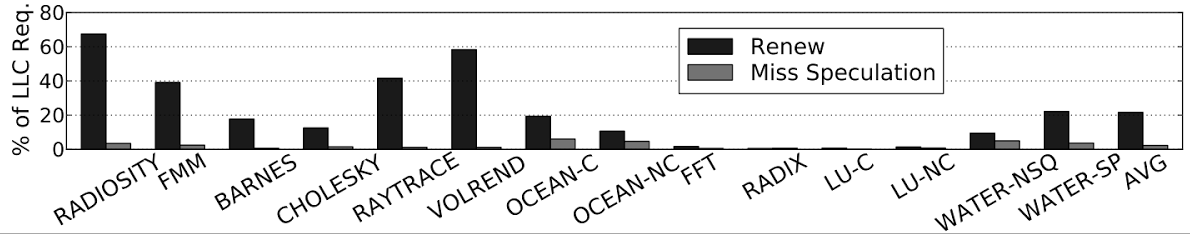
\includegraphics[width=16cm]{image1.png}
  \caption{Graph illustrating the percentage of renew requests and miss speculations (requests that actually necessary) for various benchmarks. }
  \label{fig:renewals}
\end{center}
\end{figure}

With these observations in mind, we notice that write-intensive lines should have very small lease sizes so that when renew requests are sent, we prevent prolific increase in timestamps. On the other hand, since renewing is unnecessary in read-only lines, there is a potential for much larger leases.
The basic implementation idea is that if data is renewed, then we progressively give the cacheline a smaller lease whereas data that are suspected to be read-only are incrementally given longer leases, for later renewals. In order to maintain these lease states, we add an $n$-bit counter to the cacheline that will keep track of a particular line’s “state.” Thus, if $n$ is 2, for example, four states exist, namely 00, 01, 10, and 11. 

Since this lease protocol is a very broad idea, we developed implementations that require several parameters, or different variations. One parameter is the value of $n$. If $n$ is larger, this could allow for a more calibrated lease predictor, as the number of states increases exponentially, but also creates much more storage overhead (extra $n$ bits per cacheline). Another choice is either decrementing the state progressively when a line requests exclusive ownership (10 $\rightarrow$ 01) or clearing the state counter immediately (10 $\rightarrow$ 00). In either case though, if a lease expires, we increment the state from 00 to 01, for example. The third parameter to be examined is the mapping from state to the actual lease. We have two basic algorithms, one is an exponentially growing lease and the other is a linearly growing one. Both are similar in nature, and revolve around the same ideas previously mentioned, but increase differently, as evident from the names. We also investigate the effect of using different start points for the lease (the lease assigned to 00), and the increase factor (how much a previous lease is added, or multiplied by). The sweep studies for these parameters can be found in \cref{sec:lease-prediction}.

\section{Methodology}

We used the Graphite simulator~\cite{graphite} to model our multicore 
architecture. Graphite is able to simulate 
systems with up to 1000 cores. In this report, we only simulate a 
64-core system, which matches the latest Intel multicore 
processor~\cite{xeonphi}. Each core has a 32~kB private cache and all 
cores share a 8~MB shared cache. All the cores and caches are 
connected using an on-chip network with MESH topology.

\begin{table}
	\caption{ Default Configuration of Tardis. }
	\begin{center}
	{ 
		\begin{tabular}{|l|l|}
            \hline
			\multicolumn{2}{|c|}{Timestamp Compression} \\
			\hline
			Delta timestamp size 		& 20~bits \\
			L1 Rebase Overhead 			& 128~ns\\
			L2 Rebase Overhead			& 1024~ns \\
			\hline
			\multicolumn{2}{|c|}{Livelock Detection} \\
			\hline
			Livelock detection 			& turned on \\
			Self increment period 		& 1000 \\
			\hline
			\multicolumn{2}{|c|}{Lease Prediction} \\
			\hline
			Lease prediction			& turned on \\
			Start lease 				& 8 \\
			Increase factor				& 2 \\
			\hline
		\end{tabular}
    }
	\end{center}
    \label{tab:system}
	\vspace{-.2in}
\end{table}

\cref{tab:system} shows the default configuration of Tardis. All the 
three optimizations introduced in \cref{sec:optimization} are turned 
on by default. The default delta timestamp size is 20~bits. The 
<<<<<<< HEAD
rebased overhead for L1 and L2 cache is 128~ns and 1024~ns 
respectively. During this  time, the cache is not able to serve 
=======
rebase overhead for the L1 and L2 cache is 128~ns and 1024~ns 
respectively. During this rebase time, the cache is not able to serve 
>>>>>>> 74bd8504d2d327a968e42c29a1ade675e5727e27
other requests. The default self increment period is chosen to be 
1000. The start lease is 8 for each cacheline and the increase factor 
is 2. Unless otherwise stated, all the experiments use these 
parameters by default.

We use a subset of Splash-2~\cite{splash2} benchmarks to evaluate our 
optimization techniques. For each experiment, we show the speedup, or throughput (in 
bars) and the renew rate (in red dots) for each benchmark.

\section{Evaluations}

In this section, we evaluate the performance of the optimization 
techniques introduced in \cref{sec:optimization}.

\subsection{Main Result}

\begin{figure}
	\centering
	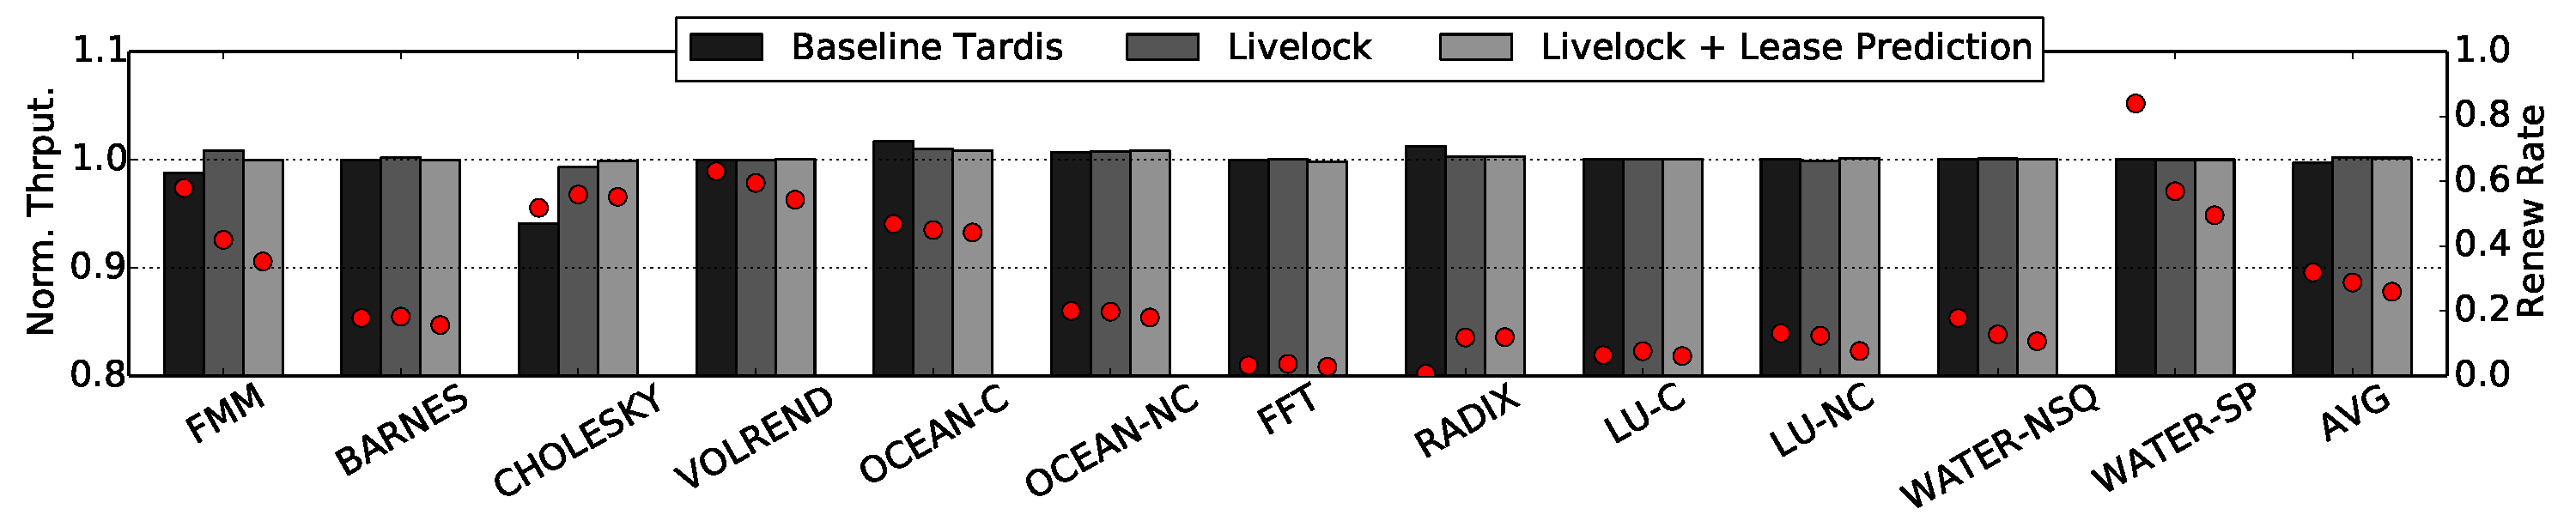
\includegraphics[width=0.95\columnwidth]{figs/main.pdf}
	\caption{ Tardis with different optimization techniques.}
	\label{fig:main}
\end{figure}

\cref{fig:main} summarizes the performance improvement of the 
optimization techniques introduced in this report. Here we show the 
performance of the baseline directory protocol, the baseline Tardis 
protocol~\cite{yu2015}, the baseline Tardis with livelock 
detection~\cref{sec:livelock-detection} and Tardis with both livelock 
detection and lease prediction~\cref{sec:lease-prediction}.

Points to discuss

- Livelock detection improves performance for benchmarks heavily using 
  spinning.

- Both livelock detection and lease prediction reduce renew rate and 
  network traffic.
  
  


\subsection{Timestamp Compression}

\begin{figure}
	\centering
	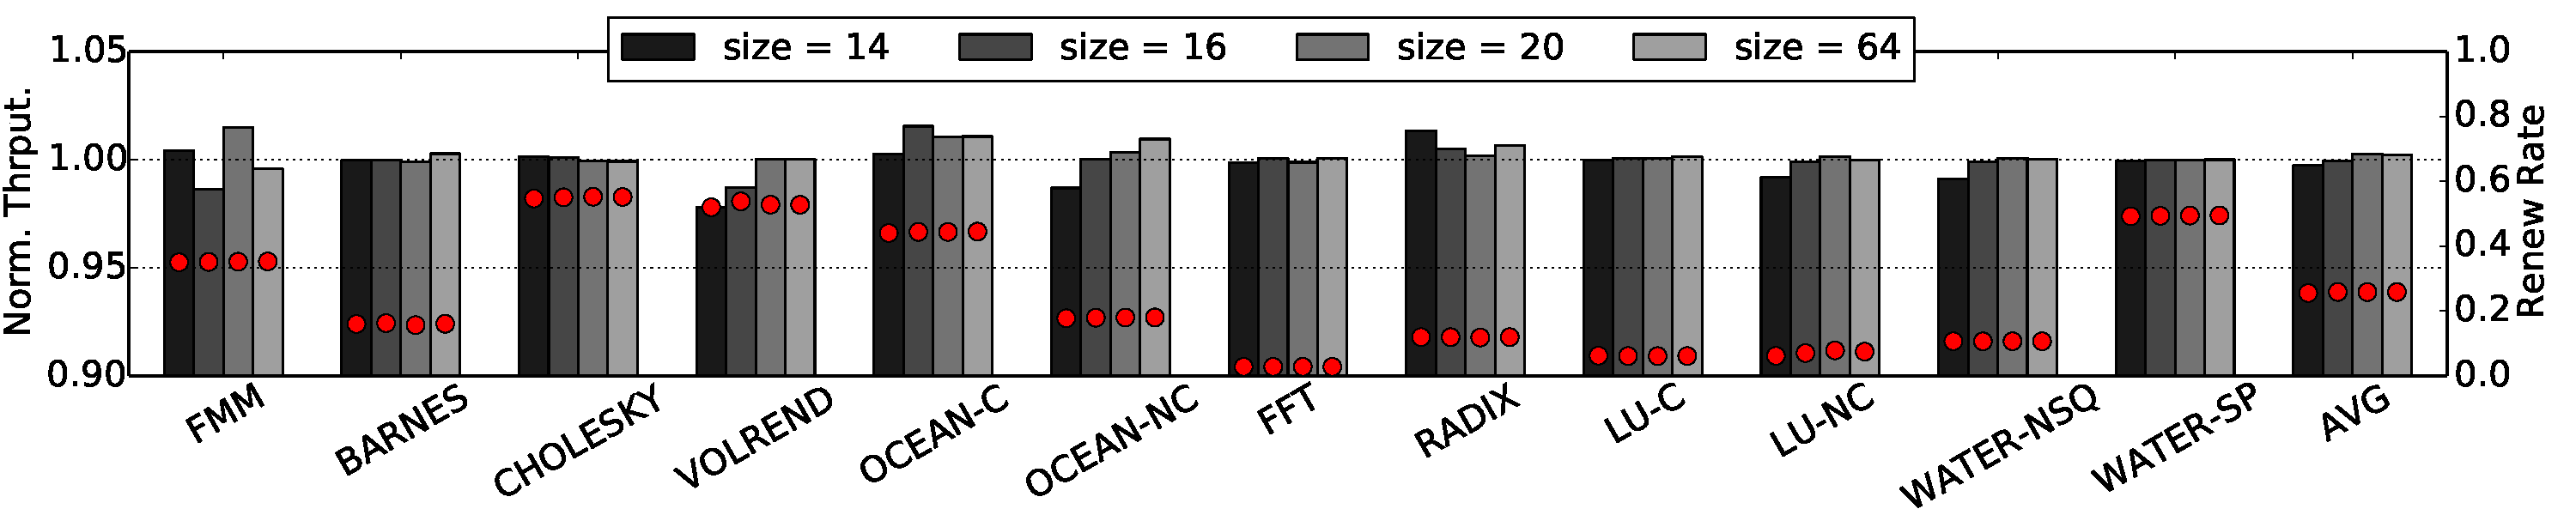
\includegraphics[width=0.95\textwidth]{figs/tssize.pdf}
	\caption{ Performance of Tardis sweeping the delta timestamp size}
	\label{fig:tssize}
\end{figure}

Please cover at least the following points in \cref{fig:tssize}:

- size = 14 has bad performance because of frequent rebase.

- As long as delta timestamp size is large enough, performance is not 
  sensitive to the timestamp size.

- We chose size = 20 as the default value since it provides reasonable 
  performance over all benchmarks.


A delta that was too small would mean frequent rebasing and lower performance while a delta too large would cause this optimization to be ineffective. Through our benchmarking tests with various delta sizes, we found a size of 14 bits had bad performance. 16 Bits was better, but we chose 20 bits in the end because it was the smallest value that had no noticeable impact on performance. Figure 4 shows that  there is noticeable performance gain when increasing the delta size from 14 to 16 to 20, but the difference between 20 bits and 64 bits is insignificant when considering the large difference in the storage size. As long as the delta size is large enough to prevent overly frequent rebasing, performance is not sensitive to timestamp size, which makes 20 bits our optimal value for the delta timestamp size
\subsection{Livelock Detection}

\begin{figure}
	\centering
	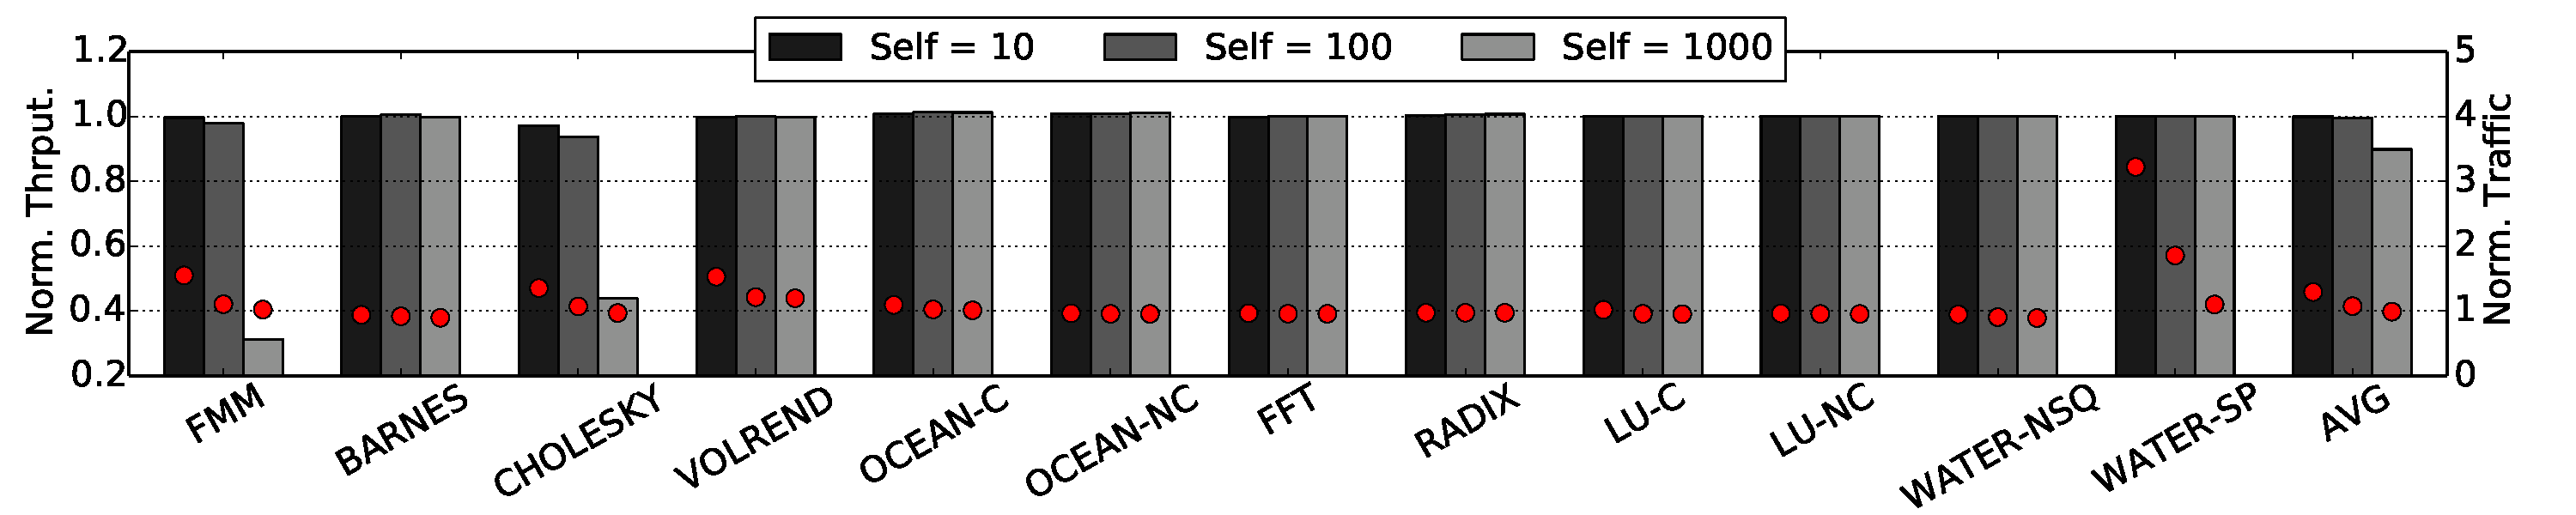
\includegraphics[width=0.95\columnwidth]{figs/selfincr_nolive.pdf}
	\caption{ Baseline Tardis without livelock detection. }
	\label{fig:self-nolive}
\end{figure}

For \cref{fig:self-nolive}, at least discuss the following points:

- For baseline Tardis, both performance and renew rate go down as self
  increment period increases. Performance goes down for some
  benchmarks because of spinning.
  
  We studied the self increment method by changing the self increment period, which is the amount of cpu cycles that the core goes though per 1 pts increment (?) . As seen with figure 5, a low self increment period resulted in higher network traffic because of frequent renew requests while a larger period decreased the renew rate but resulted in a lower performance since a livelock took longer to resolve.  
  
  
  By implementing the livelock detection system, we eliminated the decrease in performance while maintaining the gains of lower renewals and reduced network traffic.  A larger self increment period does not hurt performance anymore because our optimization deals with the livelock  as soon as it occurs by detecting it and renewing the relevant cachelines. The core no longer has to wait for self increment to for those cachelines to expire and that is what results in the lack of performance loss from large self increment periods.

\begin{figure}
	\centering
	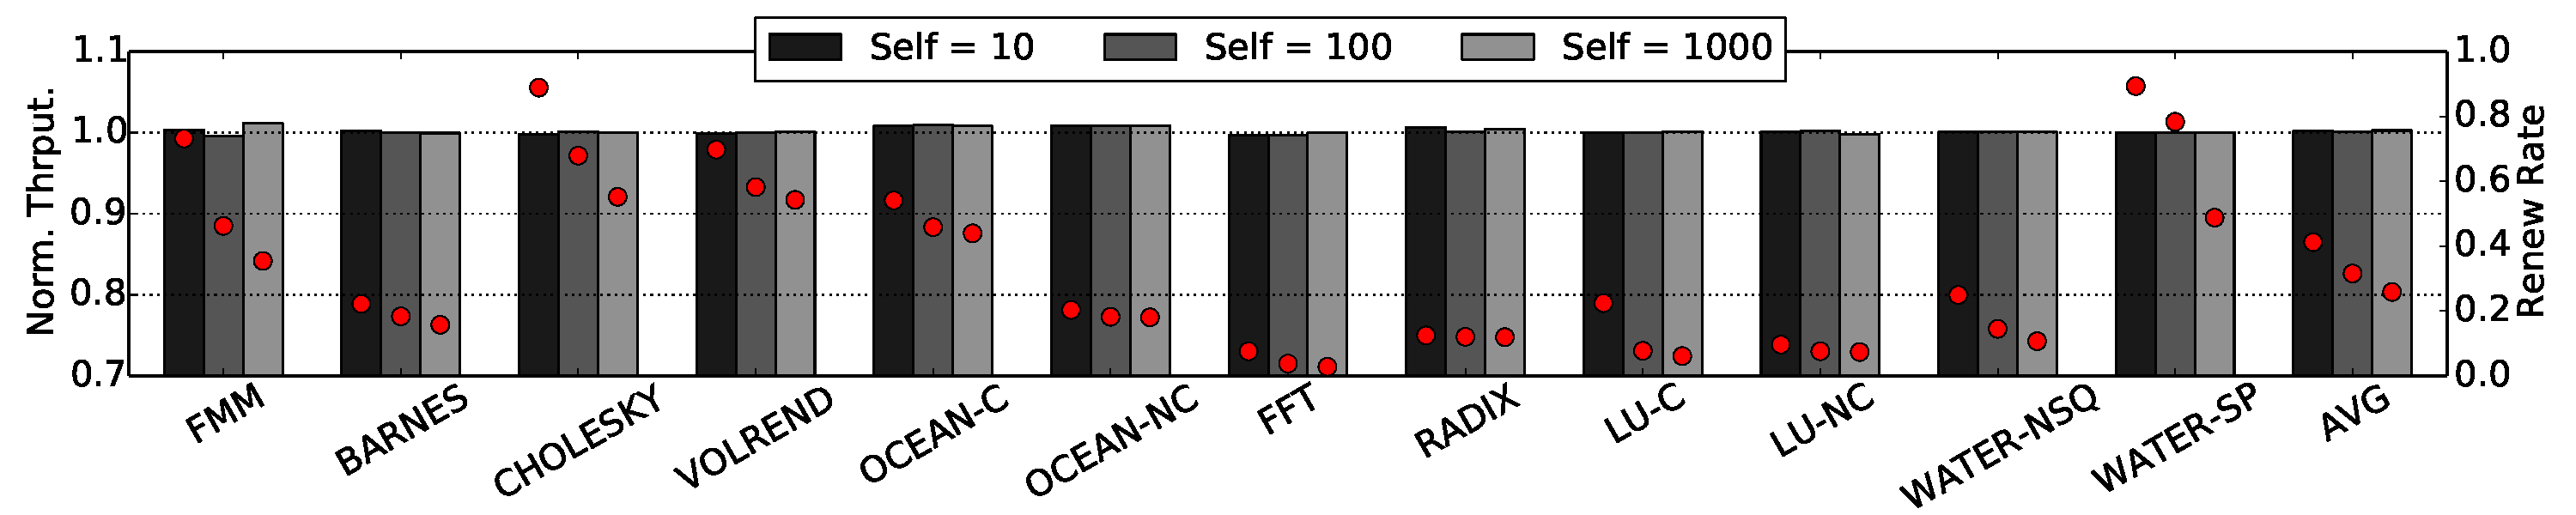
\includegraphics[width=0.95\columnwidth]{figs/selfincr_live.pdf}
	\caption{ Tardis with livelock detection. }
	\label{fig:self-live}
\end{figure}

For \cref{fig:self-live}, at least discuss the following:

- the renew messages in this experiment contains both renewals and 
  checks.

- Similar to \cref{fig:self-nolive}, increasing the self increment 
  period reduces the renew rate and network traffic. However, larger 
  self increment period does not hurt performance, because blabla...

\subsection{Lease Prediction}

\begin{figure}
	\centering
	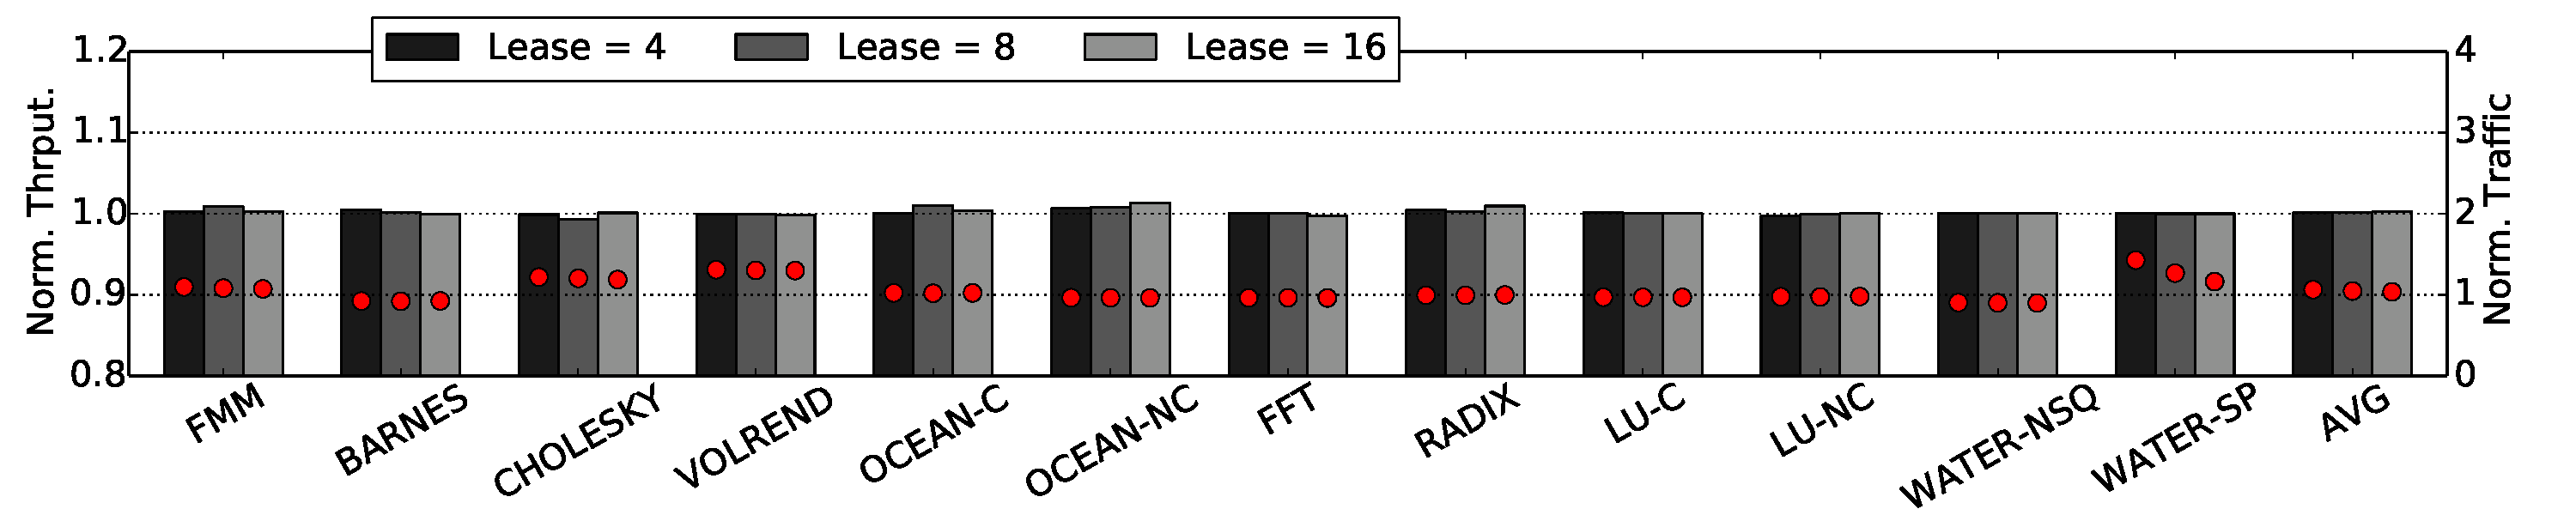
\includegraphics[width=0.95\columnwidth]{figs/static.pdf}
	\caption{ Sweeping the static lease.  }
	\label{fig:static}
\end{figure}

\cref{fig:static} sweeps the static lease from 4 to 16. Livelock 
detection is enabled in this experiment. Discuss the following points:

- performance is not sensitive to the value of static lease. However, 
  this is because we enabled livelock detection. Without livelock 
  detection, performance drops with large lease values for benchmarks 
  heavily use spinning.

- renew rate slightly reduces for most benchmarks because of less 
  renew requests.

\begin{figure}
	\centering
	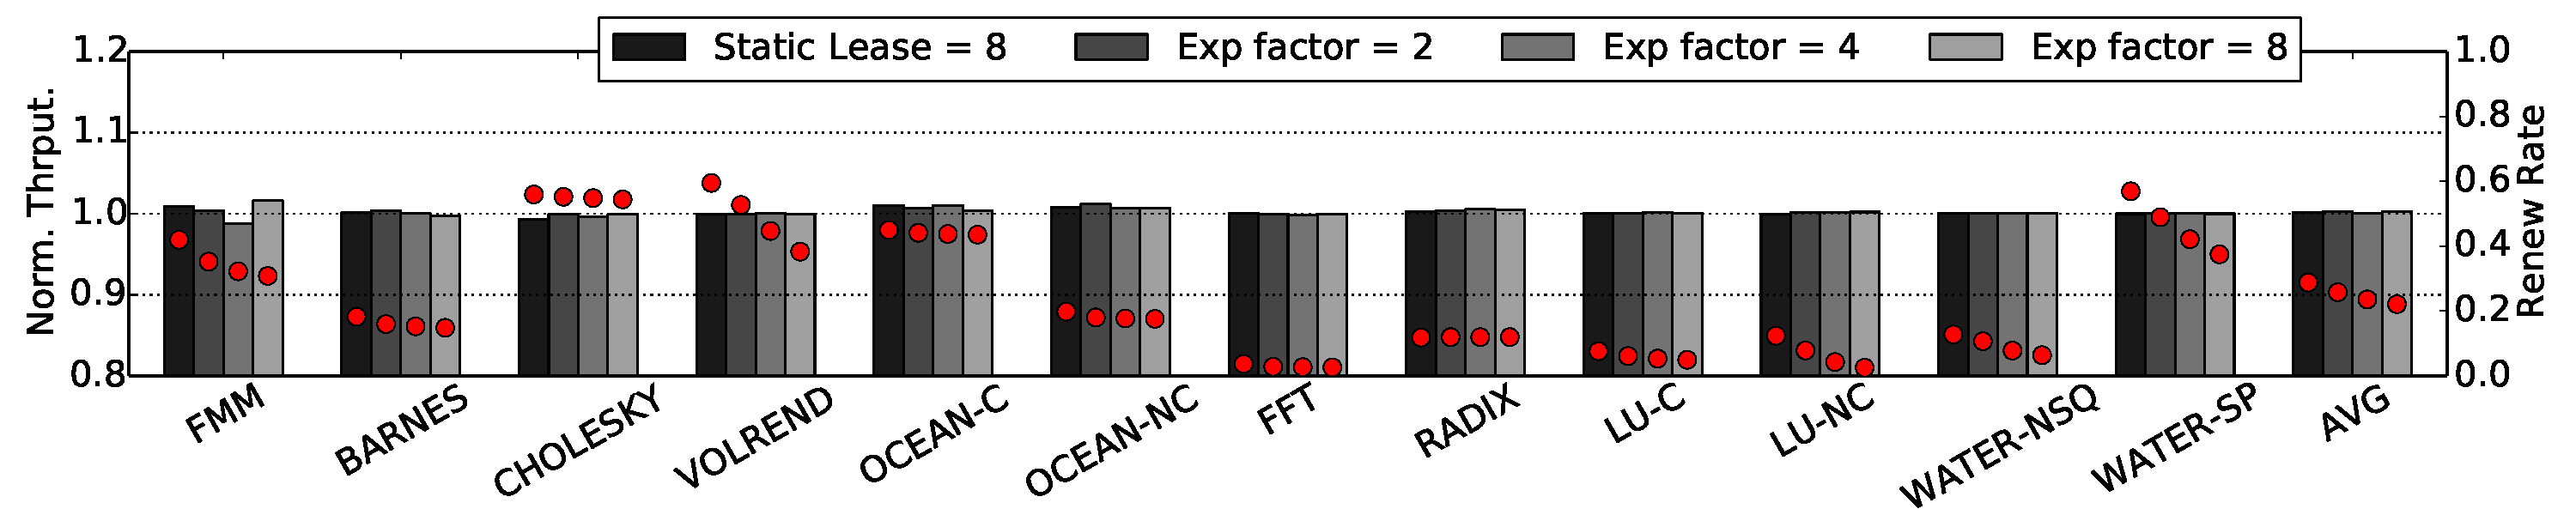
\includegraphics[width=0.95\columnwidth]{figs/exp.pdf}
	\caption{ Sweeping the increase factor for lease prediction 
	algorithm.}
	\label{fig:exp}
\end{figure}

\cref{fig:exp} shows the performance of our lease prediction algorithm 
discussed in \cref{sec:lease-prediction}. Discuss the following 
points:

- lease prediction algorithm does not affect throughput.

- lease prediction reduces renewal rate and network traffic. The 
  reduction is more significant than simply using a larger static 
  lease (\cref{fig:static}).



\section{Conclusion}
	Tardis is a new scheme to ensure memory coherence. Its main advantages are its scalability, simplicity, and to perform operations that “travel in time.” It uses logical time by incorporating timestamps in cachelines and cores. We tested multiple optimizations involving timestamp compression, lease prediction, and livelock detection, and were successful in increasing Tardis’s speed and efficiency overall (we should run a test to comepare baseline Tardis with all of our optimizations). We tested a variety of benchmarks on 64 core simulated machines via the Graphite simulator on MIT CSAIL’s Cagnode servers.

{
	\bibliographystyle{abbrv}
	\bibliography{refs}
}
\end{document}

